% !TeX program = xelatex

\documentclass{article}

\usepackage{xcolor}
\definecolor{cgreen}{rgb}{0,0.6,0}
\definecolor{cgray}{rgb}{0.5,0.5,0.5}
\definecolor{cpurple}{rgb}{0.58,0,0.82}

\usepackage{forest}

\usepackage{tikz}
\usetikzlibrary{matrix, positioning}

\tikzset{
node distance=1.4in,
State/.style={
 	draw, circle,
	align=center,
	fill=cgray
},
MarkedState/.style={
 	State,
	fill=cgreen
},
WaitedState/.style={
 	State,
	fill=black!60!red
},
Edge/.style={
	draw=black
},
MarkedEdge/.style={
	Edge,
	red
},
level/.style={
	draw, 
	minimum width=1.5cm, 
	minimum height=8mm
},
stack/.style={
	matrix of nodes, 
	nodes={level}, 
	row sep=-\pgflinewidth
}
}

\usepackage{listings}

\usepackage{mathtools}

\DeclarePairedDelimiter\abs{\lvert}{\rvert}
\DeclarePairedDelimiter\norm{\lVert}{\rVert}

\usepackage[left=1in, right=1in, top=1in, bottom=1in]{geometry}

\usepackage{diagbox}

\usepackage{fancyhdr}
\pagestyle{fancy}

\fancyhead[R]{
تمرین سری دوم هوش مصنوعی
}

\usepackage{xepersian}
\settextfont{XB Niloofar}

\begin{document}
\section*{سوال اول}
\subsection*{الف)}
با توجه به قابل قبول بودن $h$ و $g$ و با فرض اینکه 
$h^*$
هزینه اصلی باشد داریم
\begin{align*}
	\left.\begin{array}{l}
		h(n) \leq h^*(n)\\[1ex]
		g(n) \leq h^*(n)
	\end{array}\right\} \Longrightarrow\ h(n) + g(n) \leq 2 h^*(n) \Longrightarrow\ \frac{h(n) + g(n)}{2} \leq h^*(n)
\end{align*}
که به همان معنای قابل قبول بودن $ \frac{h(n) + g(n)}{2}$ است.

\subsection*{ب)}
از آنجایی که الگوریتم هزینه یکنواخت بر اساس هزینه شروع به گسترش نود‌ها می‌دهد نه عمق بنابر این با اضافه کردن $C$ به هزینه حرکت در هر مرحله به هزینه رسیدن به نودی در عمق $n$ام هزینه $(n-1)C$ اضافه می‌شود که می‌تواند باعث شود الگوریتم نود‌هایی با عمق کمتر را ترجیح دهد و به عنوان جواب پیدا کند.

\subsection*{پ)}
به ازای هر نود $n$ می‌توان گفت اگر مسیر بهینه حرکت از $n$ به هدف 
$(n_1, n_2, \cdots, n_k)$
باشد که $n_1$ همان $n$ و  کمترین هزینه حرکت از $n$ به هدف یا همان $h^*(n)$ برابر با
$\sum_{i=1}^{k-1} cost(n_i, n_{i+1})$
است.

با توجه به این و اینکه در هر مرحله
$h(n_i) \leq h(n_{i+1}) + cost(n_i, n_{i+1})$
داریم
\begin{align*}
\sum_{i=1}^{k-1} h(n_i) \leq &\sum_{i=1}^{k-1} \left[ h(n_{i+1}) + cost(n_i, n_{i+1}) \right] = h^*(n) + \sum_{i=1}^{k-1} h(n_{i+1}) \\
\Rightarrow\ &\sum_{i=1}^{k-1} h(n_i) - \sum_{i=1}^{k-1} h(n_{i+1}) \leq h^*(n) \\
\Rightarrow\ &h(n_1) = h(n) \leq h^*(n)
\end{align*}
که گزاره آخر همان تعریف قابل قبول بودن است.

از نظر شهودی اگر به صورت مرحله مرحله از هدف دور شویم تابع هزینه اصلی به اندازه هزینه یال اضافه می‌شود در حالی که شرط سازگاری الزام میکند که تابع هیوریستیک سازگار حداکثر به اندازه هزینه یال اضافه شود. بنابرین بدیهی است که به طور کلی تابع هیوریستیک سازگار حداکثر می‌تواند با تابع هزینه برابر شود و به صورت کلی حد پایینی از آن ارائه می‌دهد که یعنی تابع هیوریستیک سازگار، قابل قبول است.

\section*{سوال دوم}
به ازای هر نود $s$ با توجه به تعریف $max$ دو حالت داریم
\begin{align*}
\left.\begin{array}{lclcl}
	h_1(s) \leq h_2(s) & \rightarrow & h_3(s) = h_2(s) & \rightarrow & h_3(s) \leq h^*(s) \\[1ex]
	h_2(s) \le h_1(s) & \rightarrow & h_3(s) = h_1(s) & \rightarrow &  h_3(s) \leq h^*(s)
\end{array}\right\} \Rightarrow\ h_3(s) \leq h^*(s)
\end{align*}

\newpage
\section*{سوال سوم}
\begin{itemize}
\item
فضای حالت در اینجا از مجموعه تمام حالت‌ها، تمام حالت‌هایی که دو ربات متفاوت در یک جدول $N \times N$ می‌توانند قرار بگیرند، و مجموعه تمام حرکت‌ها (\lr{actions}) ممکن برای هر دو ربات در هر کدام از حالت‌ها، که به ازای حالت‌های مختلف بین ۱۰ تا ۶ حرکت است، تشکیل می‌شود.

\item
تعداد نود‌های فضای حالت برابر با تمام حالاتی است که دو ربات در یک جدول $N \times N$ می‌توانند قرار بگیرند، (از آنجایی که هر دو ربات می‌توانند در یک خانه حضور داشته باشند، همان حالت نهایی مسئله، پس مسئله جایشگت با جایگذاری است. در صورتی که در هر خانه امکان حضور بیشتر از یک ربات نباشد $N^2$ حالت از حالات فعلی کمتر می‌شود.) که برابر است با 
\begin{align*}
	(N \times N) \times (N \times N) = N^4
\end{align*}

تعداد یال‌های بین حالت‌ها برای حالت‌های مختلف، متفاوت است. به طور کلی اگر رباتی در یکی از چهار گوشه جدول باشه، ۳ حرکت، اگر در کنار ضلع باشد، ۴ حرکت و در غیر این صورت ۵ حرکت ممکنه خواهد داشت. پس هر دو ربات به صورت حداکثری ۱۰ حالت دارند. بنابرین تعداد یال‌های فضای حالت کمتر از 
$10 \norm{V} = 10 N^4$
است. پس فضای حالت حداکثر از $N^4$  راس و $10N^4$ یال تشکیل شده است.
 
\item 
ماکزیمم فاکتور انشعاب، حداکثر تعداد فرزندان یک راس، در اینجا با توجه به توضیحات قبل ۱۰ است.

\item
برای اینکه بررسی کنیم حالتی حالت نهایی است، کافی است موقعیت مکانی‌ ربات‌های جدول را از نظر تساوی بررسی کنیم.
همچنین به سادگی می‌توان مجموعه حالت‌های پایانی را هم تشکیل داد.
\end{itemize}

\newpage
\section*{سوال چهارم}
\subsection*{الف)}

\subsection*{DFS}

  
پیمایش را از نود $A$ شروع می‌کنیم
\begin{enumerate}
\item 
فرزند اول راس $A$، $B$  است. بنابرین ابتدا آن پیمایش می‌شود.
\begin{latin}
\begin{tikzpicture}
\node (graph) at (0, 0) {
	\begin{tikzpicture}
	\node[MarkedState] (B) {$B$ \\ $h=6$};
	\node[State, below left of=B, xshift=1.5cm, yshift=-1cm] (E) {$E$ \\ $h=12$};
	\node[State, below right of=B] (F) {$F$ \\ $h=10$};
	\node[MarkedState, above left of=E, xshift=-0.5cm, yshift=-0.5cm] (A) {$A$ \\ $h=10$};
	\node[State, above right of=F] (C) {$C$ \\ $h=2$};
	\node[State, below of=E] (H) {$H$ \\ $h=3$};
	\node[State, below right of=F] (J) {$J$ \\ $h=7$};
	\node[State, right of=H] (I) {$I$ \\ $h=11$};
	\node[State, below of=A] (D) {$D$ \\ $h=8$};
	\node[State, below right of=C] (G) {$Goal$};
	
	\draw[MarkedEdge] (A) -- node[above] {6} (B);
	\draw[Edge] (A) -- node[right] {10} (D);
	\draw[Edge] (B) -- node[above] {9} (C);
	\draw[Edge] (B) -- node[right] {5} (E);
	\draw[Edge] (B) -- node[right] {5} (I.north);
	\draw[Edge] (C) -- node[above left] {9} (F);
	\draw[Edge] (C) -- node[above right] {6} (G);
	\draw[Edge] (D) -- node[above left] {6} (E);
	\draw[Edge] (D) -- node[above right] {7} (I.north);
	\draw[Edge] (D) -- node[below] {5} (H);
	\draw[Edge] (E) -- node[below] {2} (F);
	\draw[Edge] (F) -- node[below] {5} (G);
	\draw[Edge] (F) -- node[right] {1} (I.north);
	\draw[Edge] (G) -- node[below] {9} (J);
	\draw[Edge] (H) -- node[below] {8} (I.west);
	\draw[Edge] (I) -- node[below] {3} (J);
	\end{tikzpicture}
};

\matrix[stack, label={[font=\large, align=center, name=aux1]above:{Stack}}, xshift=-2cm] (stack) at (graph.west) {
\ \\
\ \\
\ \\
B\\
A\\
};
\end{tikzpicture}
\end{latin}

\item
عمیق ترین راس پیمایش شده $B$ است و اولین فرزند آن $C$ است.
\begin{latin}
\begin{tikzpicture}
\node (graph) at (0, 0) {
	\begin{tikzpicture}
	\node[MarkedState] (B) {$B$ \\ $h=6$};
	\node[State, below left of=B, xshift=1.5cm, yshift=-1cm] (E) {$E$ \\ $h=12$};
	\node[State, below right of=B] (F) {$F$ \\ $h=10$};
	\node[MarkedState, above left of=E, xshift=-0.5cm, yshift=-0.5cm] (A) {$A$ \\ $h=10$};
	\node[MarkedState, above right of=F] (C) {$C$ \\ $h=2$};
	\node[State, below of=E] (H) {$H$ \\ $h=3$};
	\node[State, below right of=F] (J) {$J$ \\ $h=7$};
	\node[State, right of=H] (I) {$I$ \\ $h=11$};
	\node[State, below of=A] (D) {$D$ \\ $h=8$};
	\node[State, below right of=C] (G) {$Goal$};
	
	\draw[MarkedEdge] (A) -- node[above] {6} (B);
	\draw[Edge] (A) -- node[right] {10} (D);
	\draw[MarkedEdge] (B) -- node[above] {9} (C);
	\draw[Edge] (B) -- node[right] {5} (E);
	\draw[Edge] (B) -- node[right] {5} (I.north);
	\draw[Edge] (C) -- node[above left] {9} (F);
	\draw[Edge] (C) -- node[above right] {6} (G);
	\draw[Edge] (D) -- node[above left] {6} (E);
	\draw[Edge] (D) -- node[above right] {7} (I.north);
	\draw[Edge] (D) -- node[below] {5} (H);
	\draw[Edge] (E) -- node[below] {2} (F);
	\draw[Edge] (F) -- node[below] {5} (G);
	\draw[Edge] (F) -- node[right] {1} (I.north);
	\draw[Edge] (G) -- node[below] {9} (J);
	\draw[Edge] (H) -- node[below] {8} (I.west);
	\draw[Edge] (I) -- node[below] {3} (J);
	\end{tikzpicture}
};

\matrix[stack, label={[font=\large, align=center, name=aux1]above:{Stack}}, xshift=-2cm] (stack) at (graph.west) {
\ \\
\ \\
C\\
B\\
A\\
};
\end{tikzpicture}
\end{latin}

\newpage
\item
عمیق ترین راس پیمایش شده $C$ است و اولین فرزند آن $F$ است.
\begin{latin}
\begin{tikzpicture}
\node (graph) at (0, 0) {
	\begin{tikzpicture}
	\node[MarkedState] (B) {$B$ \\ $h=6$};
	\node[State, below left of=B, xshift=1.5cm, yshift=-1cm] (E) {$E$ \\ $h=12$};
	\node[MarkedState, below right of=B] (F) {$F$ \\ $h=10$};
	\node[MarkedState, above left of=E, xshift=-0.5cm, yshift=-0.5cm] (A) {$A$ \\ $h=10$};
	\node[MarkedState, above right of=F] (C) {$C$ \\ $h=2$};
	\node[State, below of=E] (H) {$H$ \\ $h=3$};
	\node[State, below right of=F] (J) {$J$ \\ $h=7$};
	\node[State, right of=H] (I) {$I$ \\ $h=11$};
	\node[State, below of=A] (D) {$D$ \\ $h=8$};
	\node[State, below right of=C] (G) {$Goal$};
	
	\draw[MarkedEdge] (A) -- node[above] {6} (B);
	\draw[Edge] (A) -- node[right] {10} (D);
	\draw[MarkedEdge] (B) -- node[above] {9} (C);
	\draw[Edge] (B) -- node[right] {5} (E);
	\draw[Edge] (B) -- node[right] {5} (I.north);
	\draw[MarkedEdge] (C) -- node[above left] {9} (F);
	\draw[Edge] (C) -- node[above right] {6} (G);
	\draw[Edge] (D) -- node[above left] {6} (E);
	\draw[Edge] (D) -- node[above right] {7} (I.north);
	\draw[Edge] (D) -- node[below] {5} (H);
	\draw[Edge] (E) -- node[below] {2} (F);
	\draw[Edge] (F) -- node[below] {5} (G);
	\draw[Edge] (F) -- node[right] {1} (I.north);
	\draw[Edge] (G) -- node[below] {9} (J);
	\draw[Edge] (H) -- node[below] {8} (I.west);
	\draw[Edge] (I) -- node[below] {3} (J);
	\end{tikzpicture}
};

\matrix[stack, label={[font=\large, align=center, name=aux1]above:{Stack}}, xshift=-2cm] (stack) at (graph.west) {
\ \\
F\\
C\\
B\\
A\\
};
\end{tikzpicture}
\end{latin}

\item
عمیق ترین راس پیمایش شده $F$ است و اولین فرزند آن $Goal$، همان هدف نهایی، است و الگوریتم خاتمه می‌یابد.
\begin{latin}
\begin{tikzpicture}
\node (graph) at (0, 0) {
	\begin{tikzpicture}
	\node[MarkedState] (B) {$B$ \\ $h=6$};
	\node[State, below left of=B, xshift=1.5cm, yshift=-1cm] (E) {$E$ \\ $h=12$};
	\node[MarkedState, below right of=B] (F) {$F$ \\ $h=10$};
	\node[MarkedState, above left of=E, xshift=-0.5cm, yshift=-0.5cm] (A) {$A$ \\ $h=10$};
	\node[MarkedState, above right of=F] (C) {$C$ \\ $h=2$};
	\node[State, below of=E] (H) {$H$ \\ $h=3$};
	\node[State, below right of=F] (J) {$J$ \\ $h=7$};
	\node[State, right of=H] (I) {$I$ \\ $h=11$};
	\node[State, below of=A] (D) {$D$ \\ $h=8$};
	\node[MarkedState, below right of=C] (G) {$Goal$};
	
	\draw[MarkedEdge] (A) -- node[above] {6} (B);
	\draw[Edge] (A) -- node[right] {10} (D);
	\draw[MarkedEdge] (B) -- node[above] {9} (C);
	\draw[Edge] (B) -- node[right] {5} (E);
	\draw[Edge] (B) -- node[right] {5} (I.north);
	\draw[MarkedEdge] (C) -- node[above left] {9} (F);
	\draw[Edge] (C) -- node[above right] {6} (G);
	\draw[Edge] (D) -- node[above left] {6} (E);
	\draw[Edge] (D) -- node[above right] {7} (I.north);
	\draw[Edge] (D) -- node[below] {5} (H);
	\draw[Edge] (E) -- node[below] {2} (F);
	\draw[MarkedEdge] (F) -- node[below] {5} (G);
	\draw[Edge] (F) -- node[right] {1} (I.north);
	\draw[Edge] (G) -- node[below] {9} (J);
	\draw[Edge] (H) -- node[below] {8} (I.west);
	\draw[Edge] (I) -- node[below] {3} (J);
	\end{tikzpicture}
};

\matrix[stack, label={[font=\large, align=center, name=aux1]above:{Stack}}, xshift=-2cm] (stack) at (graph.west) {
Goal\\
F\\
C\\
B\\
A\\
};
\end{tikzpicture}
\end{latin}
\end{enumerate}
مسر طی شده 
$(A, B, C, F, Goal)$
است در حالی که مسیر بهینه  
$(A, B, I, F, Goal)$
است بنابرین جواب بهینه نیست.

\newpage
\subsection*{BFS}

پیمایش را از نود $A$ شروع می‌کنیم
\begin{enumerate}
\item
تمام فرزندان $A$ باید به ترتیب لیست نود‌های پیمایش شده اضافه شوند.
\begin{latin}
\begin{tikzpicture}
\node (graph) at (0, 0) {
	\begin{tikzpicture}
	\node[MarkedState] (B) {$B$ \\ $h=6$};
	\node[State, below left of=B, xshift=1.5cm, yshift=-1cm] (E) {$E$ \\ $h=12$};
	\node[State, below right of=B] (F) {$F$ \\ $h=10$};
	\node[WaitedState, above left of=E, xshift=-0.5cm, yshift=-0.5cm] (A) {$A$ \\ $h=10$};
	\node[State, above right of=F] (C) {$C$ \\ $h=2$};
	\node[State, below of=E] (H) {$H$ \\ $h=3$};
	\node[State, below right of=F] (J) {$J$ \\ $h=7$};
	\node[State, right of=H] (I) {$I$ \\ $h=11$};
	\node[MarkedState, below of=A] (D) {$D$ \\ $h=8$};
	\node[State, below right of=C] (G) {$Goal$};
	
	\draw[MarkedEdge] (A) -- node[above] {6} (B);
	\draw[MarkedEdge] (A) -- node[right] {10} (D);
	\draw[Edge] (B) -- node[above] {9} (C);
	\draw[Edge] (B) -- node[right] {5} (E);
	\draw[Edge] (B) -- node[right] {5} (I.north);
	\draw[Edge] (C) -- node[above left] {9} (F);
	\draw[Edge] (C) -- node[above right] {6} (G);
	\draw[Edge] (D) -- node[above left] {6} (E);
	\draw[Edge] (D) -- node[above right] {7} (I.north);
	\draw[Edge] (D) -- node[below] {5} (H);
	\draw[Edge] (E) -- node[below] {2} (F);
	\draw[Edge] (F) -- node[below] {5} (G);
	\draw[Edge] (F) -- node[right] {1} (I.north);
	\draw[Edge] (G) -- node[below] {9} (J);
	\draw[Edge] (H) -- node[below] {8} (I.west);
	\draw[Edge] (I) -- node[below] {3} (J);
	\end{tikzpicture}
};

\matrix[stack, label={[font=\large, align=center, name=aux1]above:{To expand}}, xshift=2cm] (stack) at (graph.east) {
 B\\
D\\
};
\end{tikzpicture}
\end{latin}

\item
تمام فرزندان راس‌های $B$ و  $D$ برای بسط باید انتخاب شوند.
\begin{latin}
\begin{tikzpicture}
\node (graph) at (0, 0) {
	\begin{tikzpicture}
	\node[WaitedState] (B) {$B$ \\ $h=6$};
	\node[MarkedState, below left of=B, xshift=1.5cm, yshift=-1cm] (E) {$E$ \\ $h=12$};
	\node[State, below right of=B] (F) {$F$ \\ $h=10$};
	\node[WaitedState, above left of=E, xshift=-0.5cm, yshift=-0.5cm] (A) {$A$ \\ $h=10$};
	\node[MarkedState, above right of=F] (C) {$C$ \\ $h=2$};
	\node[MarkedState, below of=E] (H) {$H$ \\ $h=3$};
	\node[State, below right of=F] (J) {$J$ \\ $h=7$};
	\node[MarkedState, right of=H] (I) {$I$ \\ $h=11$};
	\node[WaitedState, below of=A] (D) {$D$ \\ $h=8$};
	\node[State, below right of=C] (G) {$Goal$};
	
	\draw[MarkedEdge] (A) -- node[above] {6} (B);
	\draw[MarkedEdge] (A) -- node[right] {10} (D);
	\draw[MarkedEdge] (B) -- node[above] {9} (C);
	\draw[MarkedEdge] (B) -- node[right] {5} (E);
	\draw[MarkedEdge] (B) -- node[right] {5} (I.north);
	\draw[Edge] (C) -- node[above left] {9} (F);
	\draw[Edge] (C) -- node[above right] {6} (G);
	\draw[Edge] (D) -- node[above left] {6} (E);
	\draw[MarkedEdge] (D) -- node[above right] {7} (I.north);
	\draw[MarkedEdge] (D) -- node[below] {5} (H);
	\draw[Edge] (E) -- node[below] {2} (F);
	\draw[Edge] (F) -- node[below] {5} (G);
	\draw[Edge] (F) -- node[right] {1} (I.north);
	\draw[Edge] (G) -- node[below] {9} (J);
	\draw[Edge] (H) -- node[below] {8} (I.west);
	\draw[Edge] (I) -- node[below] {3} (J);
	\end{tikzpicture}
};

\matrix[stack, label={[font=\large, align=center, name=aux1]above:{To expand}}, xshift=2cm] (stack) at (graph.east) {
C\\
E\\
H\\
I\\
};
\end{tikzpicture}
\end{latin}

\newpage
\item
تمام فرزندان راس‌های بسط داده شده قبلی برای بسط باید انتخاب شوند.
\begin{latin}
\begin{tikzpicture}
\node (graph) at (0, 0) {
	\begin{tikzpicture}
	\node[WaitedState] (B) {$B$ \\ $h=6$};
	\node[WaitedState, below left of=B, xshift=1.5cm, yshift=-1cm] (E) {$E$ \\ $h=12$};
	\node[MarkedState, below right of=B] (F) {$F$ \\ $h=10$};
	\node[WaitedState, above left of=E, xshift=-0.5cm, yshift=-0.5cm] (A) {$A$ \\ $h=10$};
	\node[WaitedState, above right of=F] (C) {$C$ \\ $h=2$};
	\node[WaitedState, below of=E] (H) {$H$ \\ $h=3$};
	\node[MarkedState, below right of=F] (J) {$J$ \\ $h=7$};
	\node[WaitedState, right of=H] (I) {$I$ \\ $h=11$};
	\node[WaitedState, below of=A] (D) {$D$ \\ $h=8$};
	\node[MarkedState, below right of=C] (G) {$Goal$};
	
	\draw[MarkedEdge] (A) -- node[above] {6} (B);
	\draw[MarkedEdge] (A) -- node[right] {10} (D);
	\draw[MarkedEdge] (B) -- node[above] {9} (C);
	\draw[MarkedEdge] (B) -- node[right] {5} (E);
	\draw[MarkedEdge] (B) -- node[right] {5} (I.north);
	\draw[MarkedEdge] (C) -- node[above left] {9} (F);
	\draw[MarkedEdge] (C) -- node[above right] {6} (G);
	\draw[Edge] (D) -- node[above left] {6} (E);
	\draw[MarkedEdge] (D) -- node[above right] {7} (I.north);
	\draw[MarkedEdge] (D) -- node[below] {5} (H);
	\draw[Edge] (E) -- node[below] {2} (F);
	\draw[Edge] (F) -- node[below] {5} (G);
	\draw[Edge] (F) -- node[right] {1} (I.north);
	\draw[Edge] (G) -- node[below] {9} (J);
	\draw[Edge] (H) -- node[below] {8} (I.west);
	\draw[MarkedEdge] (I) -- node[below] {3} (J);
	\end{tikzpicture}
};

\matrix[stack, label={[font=\large, align=center, name=aux1]above:{To expand}}, xshift=2cm] (stack) at (graph.east) {
F\\
Goal\\
J\\
};
\end{tikzpicture}
\end{latin}

\item
از آنجایی که در مرحله بعد هدف نهایی دیده می‌شود، پس الگوریتم همین جا خاتمه می‌یابد. 
راسی که $Goal$ را به عنوان فرزند گسترش داده $C$ است، برای $C$ این‌کار توسط  $B$ و برای  $B$ توسط $A$ انجام شده است. بنابرین مسیر نهایی  $A$ تا $Goal$،
$(A, B, C, Goal)$
است.

\end{enumerate}

با توجه به توضیحات مسیر به دست آمده 
$(A, B, C, Goal)$
است که با مسیر بهینه تفاوت دارد.

\newpage
\subsection*{Greedy Best-first-search}
جستجو از راس $A$ آغاز می‌شود.
\begin{enumerate}
\item 
از فرزندان $A$ کمترین مقدار تابع هیوریستیک را $B$ دارد پس گسترش می‌یابد.
\begin{latin}
\begin{tikzpicture}
\node (graph) at (0, 0) {
	\begin{tikzpicture}
	\node[MarkedState] (B) {$B$ \\ $h=6$};
	\node[State, below left of=B, xshift=1.5cm, yshift=-1cm] (E) {$E$ \\ $h=12$};
	\node[State, below right of=B] (F) {$F$ \\ $h=10$};
	\node[MarkedState, above left of=E, xshift=-0.5cm, yshift=-0.5cm] (A) {$A$ \\ $h=10$};
	\node[State, above right of=F] (C) {$C$ \\ $h=2$};
	\node[State, below of=E] (H) {$H$ \\ $h=3$};
	\node[State, below right of=F] (J) {$J$ \\ $h=7$};
	\node[State, right of=H] (I) {$I$ \\ $h=11$};
	\node[State, below of=A] (D) {$D$ \\ $h=8$};
	\node[State, below right of=C] (G) {$Goal$};
	
	\draw[MarkedEdge] (A) -- node[above] {6} (B);
	\draw[Edge] (A) -- node[right] {10} (D);
	\draw[Edge] (B) -- node[above] {9} (C);
	\draw[Edge] (B) -- node[right] {5} (E);
	\draw[Edge] (B) -- node[right] {5} (I.north);
	\draw[Edge] (C) -- node[above left] {9} (F);
	\draw[Edge] (C) -- node[above right] {6} (G);
	\draw[Edge] (D) -- node[above left] {6} (E);
	\draw[Edge] (D) -- node[above right] {7} (I.north);
	\draw[Edge] (D) -- node[below] {5} (H);
	\draw[Edge] (E) -- node[below] {2} (F);
	\draw[Edge] (F) -- node[below] {5} (G);
	\draw[Edge] (F) -- node[right] {1} (I.north);
	\draw[Edge] (G) -- node[below] {9} (J);
	\draw[Edge] (H) -- node[below] {8} (I.west);
	\draw[Edge] (I) -- node[below] {3} (J);
	\end{tikzpicture}
};

\matrix[stack, label={[font=\large, align=center, name=aux1]above:{Stack}}, xshift=-2cm] (stack) at (graph.west) {
\ \\
\ \\
B\\
A\\
};
\end{tikzpicture}
\end{latin}

\item 
از فرزندان $B$ کمترین مقدار تابع هیوریستیک را $C$ دارد پس گسترش می‌یابد.
\begin{latin}
\begin{tikzpicture}
\node (graph) at (0, 0) {
	\begin{tikzpicture}
	\node[MarkedState] (B) {$B$ \\ $h=6$};
	\node[State, below left of=B, xshift=1.5cm, yshift=-1cm] (E) {$E$ \\ $h=12$};
	\node[State, below right of=B] (F) {$F$ \\ $h=10$};
	\node[MarkedState, above left of=E, xshift=-0.5cm, yshift=-0.5cm] (A) {$A$ \\ $h=10$};
	\node[MarkedState, above right of=F] (C) {$C$ \\ $h=2$};
	\node[State, below of=E] (H) {$H$ \\ $h=3$};
	\node[State, below right of=F] (J) {$J$ \\ $h=7$};
	\node[State, right of=H] (I) {$I$ \\ $h=11$};
	\node[State, below of=A] (D) {$D$ \\ $h=8$};
	\node[State, below right of=C] (G) {$Goal$};
	
	\draw[MarkedEdge] (A) -- node[above] {6} (B);
	\draw[Edge] (A) -- node[right] {10} (D);
	\draw[MarkedEdge] (B) -- node[above] {9} (C);
	\draw[Edge] (B) -- node[right] {5} (E);
	\draw[Edge] (B) -- node[right] {5} (I.north);
	\draw[Edge] (C) -- node[above left] {9} (F);
	\draw[Edge] (C) -- node[above right] {6} (G);
	\draw[Edge] (D) -- node[above left] {6} (E);
	\draw[Edge] (D) -- node[above right] {7} (I.north);
	\draw[Edge] (D) -- node[below] {5} (H);
	\draw[Edge] (E) -- node[below] {2} (F);
	\draw[Edge] (F) -- node[below] {5} (G);
	\draw[Edge] (F) -- node[right] {1} (I.north);
	\draw[Edge] (G) -- node[below] {9} (J);
	\draw[Edge] (H) -- node[below] {8} (I.west);
	\draw[Edge] (I) -- node[below] {3} (J);
	\end{tikzpicture}
};

\matrix[stack, label={[font=\large, align=center, name=aux1]above:{Stack}}, xshift=-2cm] (stack) at (graph.west) {
\ \\
C\\
B\\
A\\
};
\end{tikzpicture}
\end{latin}

\newpage
\item 
حالت هدف یکی از فرزندان $C$ است بنابرین $Goal$ گسترش یافته و الگوریتم خاتمه می‌یابد.
\begin{latin}
\begin{tikzpicture}
\node (graph) at (0, 0) {
	\begin{tikzpicture}
	\node[MarkedState] (B) {$B$ \\ $h=6$};
	\node[State, below left of=B, xshift=1.5cm, yshift=-1cm] (E) {$E$ \\ $h=12$};
	\node[State, below right of=B] (F) {$F$ \\ $h=10$};
	\node[MarkedState, above left of=E, xshift=-0.5cm, yshift=-0.5cm] (A) {$A$ \\ $h=10$};
	\node[MarkedState, above right of=F] (C) {$C$ \\ $h=2$};
	\node[State, below of=E] (H) {$H$ \\ $h=3$};
	\node[State, below right of=F] (J) {$J$ \\ $h=7$};
	\node[State, right of=H] (I) {$I$ \\ $h=11$};
	\node[State, below of=A] (D) {$D$ \\ $h=8$};
	\node[MarkedState, below right of=C] (G) {$Goal$};
	
	\draw[MarkedEdge] (A) -- node[above] {6} (B);
	\draw[Edge] (A) -- node[right] {10} (D);
	\draw[MarkedEdge] (B) -- node[above] {9} (C);
	\draw[Edge] (B) -- node[right] {5} (E);
	\draw[Edge] (B) -- node[right] {5} (I.north);
	\draw[Edge] (C) -- node[above left] {9} (F);
	\draw[MarkedEdge] (C) -- node[above right] {6} (G);
	\draw[Edge] (D) -- node[above left] {6} (E);
	\draw[Edge] (D) -- node[above right] {7} (I.north);
	\draw[Edge] (D) -- node[below] {5} (H);
	\draw[Edge] (E) -- node[below] {2} (F);
	\draw[Edge] (F) -- node[below] {5} (G);
	\draw[Edge] (F) -- node[right] {1} (I.north);
	\draw[Edge] (G) -- node[below] {9} (J);
	\draw[Edge] (H) -- node[below] {8} (I.west);
	\draw[Edge] (I) -- node[below] {3} (J);
	\end{tikzpicture}
};

\matrix[stack, label={[font=\large, align=center, name=aux1]above:{Stack}}, xshift=-2cm] (stack) at (graph.west) {
Goal\\
C\\
B\\
A\\
};
\end{tikzpicture}
\end{latin}
\end{enumerate}
با توجه به مقدار $Stack$ مسیر به دست آمده
$(A, B, C, Goal)$
است که با مسیر بهینه تفاوت دارد. 

\newpage
\subsection*{A*}


جستجو از راس $A$ آغاز می‌شود.

\begin{enumerate}
\item
تنها $A$ در دسترس است، پس آن برای گسترش انتخاب می‌شود.
\begin{latin}
\begin{tikzpicture}
\node (graph) at (0, 0) {
	\begin{tikzpicture}
	\node[MarkedState] (B) {$B$ \\ $h=6$ \\ $g = 12$};
	\node[State, below left of=B, xshift=1.5cm, yshift=-1cm] (E) {$E$ \\ $h=12$};
	\node[State, below right of=B] (F) {$F$ \\ $h=10$};
	\node[WaitedState, above left of=E, xshift=-0.5cm, yshift=-0.5cm] (A) {$A$ \\ $h=10$};
	\node[State, above right of=F] (C) {$C$ \\ $h=2$};
	\node[State, below of=E] (H) {$H$ \\ $h=3$};
	\node[State, below right of=F] (J) {$J$ \\ $h=7$};
	\node[State, right of=H] (I) {$I$ \\ $h=11$};
	\node[MarkedState, below of=A] (D) {$D$ \\ $h=8$ \\ $g = 18$};
	\node[State, below right of=C] (G) {$Goal$};
	
	\draw[MarkedEdge] (A) -- node[above] {6} (B);
	\draw[MarkedEdge] (A) -- node[right] {10} (D);
	\draw[Edge] (B) -- node[above] {9} (C);
	\draw[Edge] (B) -- node[right] {5} (E);
	\draw[Edge] (B) -- node[right] {5} (I.north);
	\draw[Edge] (C) -- node[above left] {9} (F);
	\draw[Edge] (C) -- node[above right] {6} (G);
	\draw[Edge] (D) -- node[above left] {6} (E);
	\draw[Edge] (D) -- node[above right] {7} (I.north);
	\draw[Edge] (D) -- node[below] {5} (H);
	\draw[Edge] (E) -- node[below] {2} (F);
	\draw[Edge] (F) -- node[below] {5} (G);
	\draw[Edge] (F) -- node[right] {1} (I.north);
	\draw[Edge] (G) -- node[below] {9} (J);
	\draw[Edge] (H) -- node[below] {8} (I.west);
	\draw[Edge] (I) -- node[below] {3} (J);
	\end{tikzpicture}
};

\matrix[stack, label={[font=\large, align=center, name=aux1]above:{Cloud}}, xshift=2cm] (cloud) at (graph.east) {
C\\
D\\
};
\end{tikzpicture}
\end{latin}

\item 
با توجه به مقادیر $g$ در $B$ و $D$، راس $B$ برای گسترش انتخاب می‌شود. مقادیر  $g$ برای بقیه فرزندان $B$ را محاسبه می‌کنیم.

\begin{latin}
\begin{tikzpicture}
\node (graph) at (0, 0) {
	\begin{tikzpicture}
	\node[WaitedState] (B) {$B$ \\ $h=6$ \\ $g = 12$};
	\node[MarkedState, below left of=B, xshift=1.5cm, yshift=-1cm] (E) {$E$ \\ $h=12$  \\ $g = 23$};
	\node[State, below right of=B] (F) {$F$ \\ $h=10$};
	\node[WaitedState, above left of=E, xshift=-0.5cm, yshift=-0.5cm] (A) {$A$ \\ $h=10$};
	\node[MarkedState, above right of=F] (C) {$C$ \\ $h=2$ \\ $g = 17$};
	\node[State, below of=E] (H) {$H$ \\ $h=3$};
	\node[State, below right of=F] (J) {$J$ \\ $h=7$};
	\node[MarkedState, right of=H] (I) {$I$ \\ $h=11$ \\ $g = 22$};
	\node[MarkedState, below of=A] (D) {$D$ \\ $h=8$ \\ $g = 18$};
	\node[State, below right of=C] (G) {$Goal$};
	
	\draw[MarkedEdge] (A) -- node[above] {6} (B);
	\draw[MarkedEdge] (A) -- node[right] {10} (D);
	\draw[MarkedEdge] (B) -- node[above] {9} (C);
	\draw[MarkedEdge] (B) -- node[right] {5} (E);
	\draw[MarkedEdge] (B) -- node[right] {5} (I.north);
	\draw[Edge] (C) -- node[above left] {9} (F);
	\draw[Edge] (C) -- node[above right] {6} (G);
	\draw[Edge] (D) -- node[above left] {6} (E);
	\draw[Edge] (D) -- node[above right] {7} (I.north);
	\draw[Edge] (D) -- node[below] {5} (H);
	\draw[Edge] (E) -- node[below] {2} (F);
	\draw[Edge] (F) -- node[below] {5} (G);
	\draw[Edge] (F) -- node[right] {1} (I.north);
	\draw[Edge] (G) -- node[below] {9} (J);
	\draw[Edge] (H) -- node[below] {8} (I.west);
	\draw[Edge] (I) -- node[below] {3} (J);
	\end{tikzpicture}
};

\matrix[stack, label={[font=\large, align=center, name=aux1]above:{Cloud}}, xshift=2cm] (cloud) at (graph.east) {
D\\
C\\
I\\
E\\
}; 

\end{tikzpicture}
\end{latin}

\newpage
\item
با توجه مقادیر $g$، راس $C$ برای گسترش انتخاب می‌شود و بعد از پیمایش $Goal$، هدف، الگوریتم پایان می‌یابد.

\begin{latin}
\begin{tikzpicture}
\node (graph) at (0, 0) {
	\begin{tikzpicture}
	\node[WaitedState] (B) {$B$ \\ $h=6$ \\ $g = 12$};
	\node[MarkedState, below left of=B, xshift=1.5cm, yshift=-1cm] (E) {$E$ \\ $h=12$  \\ $g = 23$};
	\node[State, below right of=B] (F) {$F$ \\ $h=10$};
	\node[WaitedState, above left of=E, xshift=-0.5cm, yshift=-0.5cm] (A) {$A$ \\ $h=10$};
	\node[WaitedState, above right of=F] (C) {$C$ \\ $h=2$ \\ $g = 17$};
	\node[State, below of=E] (H) {$H$ \\ $h=3$};
	\node[State, below right of=F] (J) {$J$ \\ $h=7$};
	\node[MarkedState, right of=H] (I) {$I$ \\ $h=11$ \\ $g = 22$};
	\node[MarkedState, below of=A] (D) {$D$ \\ $h=8$ \\ $g = 18$};
	\node[MarkedState, below right of=C] (G) {$Goal$};
	
	\draw[MarkedEdge] (A) -- node[above] {6} (B);
	\draw[MarkedEdge] (A) -- node[right] {10} (D);
	\draw[MarkedEdge] (B) -- node[above] {9} (C);
	\draw[MarkedEdge] (B) -- node[right] {5} (E);
	\draw[MarkedEdge] (B) -- node[right] {5} (I.north);
	\draw[MarkedEdge] (C) -- node[above left] {9} (F);
	\draw[Edge] (C) -- node[above right] {6} (G);
	\draw[Edge] (D) -- node[above left] {6} (E);
	\draw[Edge] (D) -- node[above right] {7} (I.north);
	\draw[Edge] (D) -- node[below] {5} (H);
	\draw[Edge] (E) -- node[below] {2} (F);
	\draw[Edge] (F) -- node[below] {5} (G);
	\draw[Edge] (F) -- node[right] {1} (I.north);
	\draw[Edge] (G) -- node[below] {9} (J);
	\draw[Edge] (H) -- node[below] {8} (I.west);
	\draw[Edge] (I) -- node[below] {3} (J);
	\end{tikzpicture}
};
\end{tikzpicture}
\end{latin}
\end{enumerate}

با توجه به روند گسترش راس‌ها مسیر به دست آمده 
$(A, B, C, Goal)$
است که با مسیر بهینه تفاوت دارد. از آنجایی که تابع $h$ این مسئله نه قابل قبول است نه سازگار‌ (برای مثال $h$  در راس $E$ بیشتر از $h^* = 7$ است) بهینه نبودن $A^*$ ممکن بوده است.

\newpage
\subsection*{UCS}


\begin{enumerate}
\item
ابتدا تنها راس در دسترس، راس  $A$، گسترش می‌یابد.
\begin{latin}
\begin{tikzpicture}
\node (graph) at (0, 0) {
	\begin{tikzpicture}
	\node[MarkedState] (B) {$B$ \\ $h=6$ \\ $c = 6$};
	\node[State, below left of=B, xshift=1.5cm, yshift=-1cm] (E) {$E$ \\ $h=12$};
	\node[State, below right of=B] (F) {$F$ \\ $h=10$};
	\node[WaitedState, above left of=E, xshift=-0.5cm, yshift=-0.5cm] (A) {$A$ \\ $h=10$};
	\node[State, above right of=F] (C) {$C$ \\ $h=2$};
	\node[State, below of=E] (H) {$H$ \\ $h=3$};
	\node[State, below right of=F] (J) {$J$ \\ $h=7$};
	\node[State, right of=H] (I) {$I$ \\ $h=11$};
	\node[MarkedState, below of=A] (D) {$D$ \\ $h=8$ \\ $c = 10$};
	\node[State, below right of=C] (G) {$Goal$};
	
	\draw[MarkedEdge] (A) -- node[above] {6} (B);
	\draw[MarkedEdge] (A) -- node[right] {10} (D);
	\draw[Edge] (B) -- node[above] {9} (C);
	\draw[Edge] (B) -- node[right] {5} (E);
	\draw[Edge] (B) -- node[right] {5} (I.north);
	\draw[Edge] (C) -- node[above left] {9} (F);
	\draw[Edge] (C) -- node[above right] {6} (G);
	\draw[Edge] (D) -- node[above left] {6} (E);
	\draw[Edge] (D) -- node[above right] {7} (I.north);
	\draw[Edge] (D) -- node[below] {5} (H);
	\draw[Edge] (E) -- node[below] {2} (F);
	\draw[Edge] (F) -- node[below] {5} (G);
	\draw[Edge] (F) -- node[right] {1} (I.north);
	\draw[Edge] (G) -- node[below] {9} (J);
	\draw[Edge] (H) -- node[below] {8} (I.west);
	\draw[Edge] (I) -- node[below] {3} (J);
	\end{tikzpicture}
};

\matrix[stack, label={[font=\large, align=center, name=aux1]above:{To expand}}, xshift=2cm] (stack) at (graph.east) {
 B\\
D\\
};
\end{tikzpicture}
\end{latin}

\item
از بین $B$ و $D$ کمترین هزینه را راس $B$ دارد، بنابر این گسترش میابد.
\begin{latin}
\begin{tikzpicture}
\node (graph) at (0, 0) {
	\begin{tikzpicture}
	\node[WaitedState] (B) {$B$ \\ $h=6$ \\ $c = 6$};
	\node[MarkedState, below left of=B, xshift=1.5cm, yshift=-1cm] (E) {$E$ \\ $h=12$ \\ $c = 11$};
	\node[State, below right of=B] (F) {$F$ \\ $h=10$};
	\node[WaitedState, above left of=E, xshift=-0.5cm, yshift=-0.5cm] (A) {$A$ \\ $h=10$};
	\node[MarkedState, above right of=F] (C) {$C$ \\ $h=2$ \\ $c = 17$};
	\node[State, below of=E] (H) {$H$ \\ $h=3$};
	\node[State, below right of=F] (J) {$J$ \\ $h=7$};
	\node[MarkedState, right of=H] (I) {$I$ \\ $h=11$ \\ $c = 11$};
	\node[MarkedState, below of=A] (D) {$D$ \\ $h=8$ \\ $c=10$};
	\node[State, below right of=C] (G) {$Goal$};
	
	\draw[MarkedEdge] (A) -- node[above] {6} (B);
	\draw[MarkedEdge] (A) -- node[right] {10} (D);
	\draw[MarkedEdge] (B) -- node[above] {9} (C);
	\draw[MarkedEdge] (B) -- node[right] {5} (E);
	\draw[MarkedEdge] (B) -- node[right] {5} (I.north);
	\draw[Edge] (C) -- node[above left] {9} (F);
	\draw[Edge] (C) -- node[above right] {6} (G);
	\draw[Edge] (D) -- node[above left] {6} (E);
	\draw[Edge] (D) -- node[above right] {7} (I.north);
	\draw[Edge] (D) -- node[below] {5} (H);
	\draw[Edge] (E) -- node[below] {2} (F);
	\draw[Edge] (F) -- node[below] {5} (G);
	\draw[Edge] (F) -- node[right] {1} (I.north);
	\draw[Edge] (G) -- node[below] {9} (J);
	\draw[Edge] (H) -- node[below] {8} (I.west);
	\draw[Edge] (I) -- node[below] {3} (J);
	\end{tikzpicture}
};

\matrix[stack, label={[font=\large, align=center, name=aux1]above:{To expand}}, xshift=2cm] (stack) at (graph.east) {
D\\
C\\
E\\
I\\
};
\end{tikzpicture}
\end{latin}

\newpage
\item
از بین $To\ expand$ کمترین هزینه را راس $D$ دارد.
\begin{latin}
\begin{tikzpicture}
\node (graph) at (0, 0) {
	\begin{tikzpicture}
	\node[WaitedState] (B) {$B$ \\ $h=6$ \\ $c = 6$};
	\node[MarkedState, below left of=B, xshift=1.5cm, yshift=-1cm] (E) {$E$ \\ $h=12$ \\ $c = 11$};
	\node[State, below right of=B] (F) {$F$ \\ $h=10$};
	\node[WaitedState, above left of=E, xshift=-0.5cm, yshift=-0.5cm] (A) {$A$ \\ $h=10$};
	\node[MarkedState, above right of=F] (C) {$C$ \\ $h=2$ \\ $c = 17$};
	\node[MarkedState, below of=E] (H) {$H$ \\ $h=3$ \\ $c = 15$};
	\node[State, below right of=F] (J) {$J$ \\ $h=7$};
	\node[MarkedState, right of=H] (I) {$I$ \\ $h=11$ \\ $c = 11$};
	\node[WaitedState, below of=A] (D) {$D$ \\ $h=8$ \\ $c=10$};
	\node[State, below right of=C] (G) {$Goal$};
	
	\draw[MarkedEdge] (A) -- node[above] {6} (B);
	\draw[MarkedEdge] (A) -- node[right] {10} (D);
	\draw[MarkedEdge] (B) -- node[above] {9} (C);
	\draw[MarkedEdge] (B) -- node[right] {5} (E);
	\draw[MarkedEdge] (B) -- node[right] {5} (I.north);
	\draw[Edge] (C) -- node[above left] {9} (F);
	\draw[Edge] (C) -- node[above right] {6} (G);
	\draw[Edge] (D) -- node[above left] {6} (E);
	\draw[Edge] (D) -- node[above right] {7} (I.north);
	\draw[MarkedEdge] (D) -- node[below] {5} (H);
	\draw[Edge] (E) -- node[below] {2} (F);
	\draw[Edge] (F) -- node[below] {5} (G);
	\draw[Edge] (F) -- node[right] {1} (I.north);
	\draw[Edge] (G) -- node[below] {9} (J);
	\draw[Edge] (H) -- node[below] {8} (I.west);
	\draw[Edge] (I) -- node[below] {3} (J);
	\end{tikzpicture}
};

\matrix[stack, label={[font=\large, align=center, name=aux1]above:{To expand}}, xshift=2cm] (stack) at (graph.east) {
C\\
E\\
I\\
H\\
};
\end{tikzpicture}
\end{latin}

راس $E$ برای گسترش انتخاب می‌شود.
\begin{latin}
\begin{tikzpicture}
\node (graph) at (0, 0) {
	\begin{tikzpicture}
	\node[WaitedState] (B) {$B$ \\ $h=6$ \\ $c = 6$};
	\node[WaitedState, below left of=B, xshift=1.5cm, yshift=-1cm] (E) {$E$ \\ $h=12$ \\ $c = 11$};
	\node[MarkedState, below right of=B] (F) {$F$ \\ $h=10$ \\ $c = 13$};
	\node[WaitedState, above left of=E, xshift=-0.5cm, yshift=-0.5cm] (A) {$A$ \\ $h=10$};
	\node[MarkedState, above right of=F] (C) {$C$ \\ $h=2$ \\ $c = 17$};
	\node[MarkedState, below of=E] (H) {$H$ \\ $h=3$ \\ $c = 15$};
	\node[State, below right of=F] (J) {$J$ \\ $h=7$};
	\node[MarkedState, right of=H] (I) {$I$ \\ $h=11$ \\ $c = 11$};
	\node[WaitedState, below of=A] (D) {$D$ \\ $h=8$ \\ $c=10$};
	\node[State, below right of=C] (G) {$Goal$};
	
	\draw[MarkedEdge] (A) -- node[above] {6} (B);
	\draw[MarkedEdge] (A) -- node[right] {10} (D);
	\draw[MarkedEdge] (B) -- node[above] {9} (C);
	\draw[MarkedEdge] (B) -- node[right] {5} (E);
	\draw[MarkedEdge] (B) -- node[right] {5} (I.north);
	\draw[Edge] (C) -- node[above left] {9} (F);
	\draw[Edge] (C) -- node[above right] {6} (G);
	\draw[Edge] (D) -- node[above left] {6} (E);
	\draw[Edge] (D) -- node[above right] {7} (I.north);
	\draw[MarkedEdge] (D) -- node[below] {5} (H);
	\draw[MarkedEdge] (E) -- node[below] {2} (F);
	\draw[Edge] (F) -- node[below] {5} (G);
	\draw[Edge] (F) -- node[right] {1} (I.north);
	\draw[Edge] (G) -- node[below] {9} (J);
	\draw[Edge] (H) -- node[below] {8} (I.west);
	\draw[Edge] (I) -- node[below] {3} (J);
	\end{tikzpicture}
};

\matrix[stack, label={[font=\large, align=center, name=aux1]above:{To expand}}, xshift=2cm] (stack) at (graph.east) {
C\\
I\\
H\\
F\\
};
\end{tikzpicture}
\end{latin}


\newpage
راس $I$ برای گسترش انتخاب می‌شود.
\begin{latin}
\begin{tikzpicture}
\node (graph) at (0, 0) {
	\begin{tikzpicture}
	\node[WaitedState] (B) {$B$ \\ $h=6$ \\ $c = 6$};
	\node[WaitedState, below left of=B, xshift=1.5cm, yshift=-1cm] (E) {$E$ \\ $h=12$ \\ $c = 11$};
	\node[MarkedState, below right of=B] (F) {$F$ \\ $h=10$ \\ $c = 12$};
	\node[WaitedState, above left of=E, xshift=-0.5cm, yshift=-0.5cm] (A) {$A$ \\ $h=10$};
	\node[MarkedState, above right of=F] (C) {$C$ \\ $h=2$ \\ $c = 17$};
	\node[MarkedState, below of=E] (H) {$H$ \\ $h=3$ \\ $c = 15$};
	\node[MarkedState, below right of=F] (J) {$J$ \\ $h=7$ \\ $c = 14$};
	\node[WaitedState, right of=H] (I) {$I$ \\ $h=11$ \\ $c = 11$};
	\node[WaitedState, below of=A] (D) {$D$ \\ $h=8$ \\ $c=10$};
	\node[State, below right of=C] (G) {$Goal$};
	
	\draw[MarkedEdge] (A) -- node[above] {6} (B);
	\draw[MarkedEdge] (A) -- node[right] {10} (D);
	\draw[MarkedEdge] (B) -- node[above] {9} (C);
	\draw[MarkedEdge] (B) -- node[right] {5} (E);
	\draw[MarkedEdge] (B) -- node[right] {5} (I.north);
	\draw[Edge] (C) -- node[above left] {9} (F);
	\draw[Edge] (C) -- node[above right] {6} (G);
	\draw[Edge] (D) -- node[above left] {6} (E);
	\draw[Edge] (D) -- node[above right] {7} (I.north);
	\draw[MarkedEdge] (D) -- node[below] {5} (H);
	\draw[MarkedEdge] (E) -- node[below] {2} (F);
	\draw[Edge] (F) -- node[below] {5} (G);
	\draw[MarkedEdge] (F) -- node[right] {1} (I.north);
	\draw[Edge] (G) -- node[below] {9} (J);
	\draw[Edge] (H) -- node[below] {8} (I.west);
	\draw[MarkedEdge] (I) -- node[below] {3} (J);
	\end{tikzpicture}
};

\matrix[stack, label={[font=\large, align=center, name=aux1]above:{To expand}}, xshift=2cm] (stack) at (graph.east) {
C\\
H\\
F\\
J\\
};
\end{tikzpicture}
\end{latin}

راس $F$ برای گسترش انتخاب می‌شود. با توجه به اینکه به راس هدف میرسیم الگوریتم پایان میابد.
\begin{latin}
\begin{tikzpicture}
\node (graph) at (0, 0) {
	\begin{tikzpicture}
	\node[WaitedState] (B) {$B$ \\ $h=6$ \\ $c = 6$};
	\node[WaitedState, below left of=B, xshift=1.5cm, yshift=-1cm] (E) {$E$ \\ $h=12$ \\ $c = 11$};
	\node[WaitedState, below right of=B] (F) {$F$ \\ $h=10$ \\ $c = 12$};
	\node[WaitedState, above left of=E, xshift=-0.5cm, yshift=-0.5cm] (A) {$A$ \\ $h=10$};
	\node[MarkedState, above right of=F] (C) {$C$ \\ $h=2$ \\ $c = 17$};
	\node[MarkedState, below of=E] (H) {$H$ \\ $h=3$ \\ $c = 15$};
	\node[MarkedState, below right of=F] (J) {$J$ \\ $h=7$ \\ $c = 14$};
	\node[WaitedState, right of=H] (I) {$I$ \\ $h=11$ \\ $c = 11$};
	\node[WaitedState, below of=A] (D) {$D$ \\ $h=8$ \\ $c=10$};
	\node[MarkedState, below right of=C] (G) {$Goal$ \\ $c = 17$};
	
	\draw[MarkedEdge] (A) -- node[above] {6} (B);
	\draw[MarkedEdge] (A) -- node[right] {10} (D);
	\draw[MarkedEdge] (B) -- node[above] {9} (C);
	\draw[MarkedEdge] (B) -- node[right] {5} (E);
	\draw[MarkedEdge] (B) -- node[right] {5} (I.north);
	\draw[Edge] (C) -- node[above left] {9} (F);
	\draw[Edge] (C) -- node[above right] {6} (G);
	\draw[Edge] (D) -- node[above left] {6} (E);
	\draw[Edge] (D) -- node[above right] {7} (I.north);
	\draw[MarkedEdge] (D) -- node[below] {5} (H);
	\draw[MarkedEdge] (E) -- node[below] {2} (F);
	\draw[MarkedEdge] (F) -- node[below] {5} (G);
	\draw[MarkedEdge] (F) -- node[right] {1} (I.north);
	\draw[Edge] (G) -- node[below] {9} (J);
	\draw[Edge] (H) -- node[below] {8} (I.west);
	\draw[MarkedEdge] (I) -- node[below] {3} (J);
	\end{tikzpicture}
};

\matrix[stack, label={[font=\large, align=center, name=aux1]above:{To expand}}, xshift=2cm] (stack) at (graph.east) {
C\\
H\\
J\\
Goal\\
};
\end{tikzpicture}
\end{latin}
\end{enumerate}

به سادگی می‌‌‌توان دید که مسیر به است آمده، 
$(A, B, I, F, Goal)$، مسیر بهینه است.

%\newpage
%\subsection*{RBFS}
%
%
%\begin{enumerate}
%\item 
%کمترین مقدار $g$ از فرزندان $A$ را برای پیمایش راس $B$ دارد.
%\begin{latin}
%\begin{tikzpicture}
%\node (graph) at (0, 0) {
%	\begin{tikzpicture}
%	\node[MarkedState] (B) {$B$ \\ $h=6$};
%	\node[State, below left of=B, xshift=1.5cm, yshift=-1cm] (E) {$E$ \\ $h=12$};
%	\node[State, below right of=B] (F) {$F$ \\ $h=10$};
%	\node[MarkedState, above left of=E, xshift=-0.5cm, yshift=-0.5cm] (A) {$A$ \\ $h=10$};
%	\node[State, above right of=F] (C) {$C$ \\ $h=2$};
%	\node[State, below of=E] (H) {$H$ \\ $h=3$};
%	\node[State, below right of=F] (J) {$J$ \\ $h=7$};
%	\node[State, right of=H] (I) {$I$ \\ $h=11$};
%	\node[State, below of=A] (D) {$D$ \\ $h=8$};
%	\node[State, below right of=C] (G) {$Goal$};
%	
%	\draw[MarkedEdge] (A) -- node[above] {6} (B);
%	\draw[Edge] (A) -- node[right] {10} (D);
%	\draw[Edge] (B) -- node[above] {9} (C);
%	\draw[Edge] (B) -- node[right] {5} (E);
%	\draw[Edge] (B) -- node[right] {5} (I.north);
%	\draw[Edge] (C) -- node[above left] {9} (F);
%	\draw[Edge] (C) -- node[above right] {6} (G);
%	\draw[Edge] (D) -- node[above left] {6} (E);
%	\draw[Edge] (D) -- node[above right] {7} (I.north);
%	\draw[Edge] (D) -- node[below] {5} (H);
%	\draw[Edge] (E) -- node[below] {2} (F);
%	\draw[Edge] (F) -- node[below] {5} (G);
%	\draw[Edge] (F) -- node[right] {1} (I.north);
%	\draw[Edge] (G) -- node[below] {9} (J);
%	\draw[Edge] (H) -- node[below] {8} (I.west);
%	\draw[Edge] (I) -- node[below] {3} (J);
%	\end{tikzpicture}
%};
%
%\matrix[stack, label={[font=\large, align=center, name=aux1]above:{Stack}}, xshift=-2cm] (stack) at (graph.west) {
%$B \rightarrow\  18$\\
%$A \rightarrow\  \infty$ \\
%};
%\end{tikzpicture}
%\end{latin}
%
%\item 
%از بین فرزندان $B$ تنها $C$ محدودیت $18$ را در هزینه رد نمی‌کند بنابرین این راس انتخاب می‌شود.
%\begin{latin}
%\begin{tikzpicture}
%\node (graph) at (0, 0) {
%	\begin{tikzpicture}
%	\node[MarkedState] (B) {$B$ \\ $h=6$};
%	\node[State, below left of=B, xshift=1.5cm, yshift=-1cm] (E) {$E$ \\ $h=12$};
%	\node[State, below right of=B] (F) {$F$ \\ $h=10$};
%	\node[MarkedState, above left of=E, xshift=-0.5cm, yshift=-0.5cm] (A) {$A$ \\ $h=10$};
%	\node[MarkedState, above right of=F] (C) {$C$ \\ $h=2$};
%	\node[State, below of=E] (H) {$H$ \\ $h=3$};
%	\node[State, below right of=F] (J) {$J$ \\ $h=7$};
%	\node[State, right of=H] (I) {$I$ \\ $h=11$};
%	\node[State, below of=A] (D) {$D$ \\ $h=8$};
%	\node[State, below right of=C] (G) {$Goal$};
%	
%	\draw[MarkedEdge] (A) -- node[above] {6} (B);
%	\draw[Edge] (A) -- node[right] {10} (D);
%	\draw[MarkedEdge] (B) -- node[above] {9} (C);
%	\draw[Edge] (B) -- node[right] {5} (E);
%	\draw[Edge] (B) -- node[right] {5} (I.north);
%	\draw[Edge] (C) -- node[above left] {9} (F);
%	\draw[Edge] (C) -- node[above right] {6} (G);
%	\draw[Edge] (D) -- node[above left] {6} (E);
%	\draw[Edge] (D) -- node[above right] {7} (I.north);
%	\draw[Edge] (D) -- node[below] {5} (H);
%	\draw[Edge] (E) -- node[below] {2} (F);
%	\draw[Edge] (F) -- node[below] {5} (G);
%	\draw[Edge] (F) -- node[right] {1} (I.north);
%	\draw[Edge] (G) -- node[below] {9} (J);
%	\draw[Edge] (H) -- node[below] {8} (I.west);
%	\draw[Edge] (I) -- node[below] {3} (J);
%	\end{tikzpicture}
%};
%
%\matrix[stack, label={[font=\large, align=center, name=aux1]above:{Stack}}, xshift=-2cm] (stack) at (graph.west) {
%$C \rightarrow\ 18$\\
%$B \rightarrow\ 18$\\
%$A \rightarrow\  \infty$ \\
%};
%\end{tikzpicture}
%\end{latin}
%
%\newpage
%\item
%از فرزاندان $C$ همه محدودیت هزینه را رد می‌کنند بنابرین الگوریتم به بن بست می‌خورد و برمیگردد. راس بعدی که می تواند گسترش یابد $D$ خواهد بود.
%\begin{latin}
%\begin{tikzpicture}
%\node (graph) at (0, 0) {
%	\begin{tikzpicture}
%	\node[WaitedState] (B) {$B$ \\ $h=6$};
%	\node[State, below left of=B, xshift=1.5cm, yshift=-1cm] (E) {$E$ \\ $h=12$};
%	\node[State, below right of=B] (F) {$F$ \\ $h=10$};
%	\node[MarkedState, above left of=E, xshift=-0.5cm, yshift=-0.5cm] (A) {$A$ \\ $h=10$};
%	\node[WaitedState, above right of=F] (C) {$C$ \\ $h=2$};
%	\node[State, below of=E] (H) {$H$ \\ $h=3$};
%	\node[State, below right of=F] (J) {$J$ \\ $h=7$};
%	\node[State, right of=H] (I) {$I$ \\ $h=11$};
%	\node[MarkedState, below of=A] (D) {$D$ \\ $h=8$};
%	\node[State, below right of=C] (G) {$Goal$};
%	
%	\draw[MarkedEdge] (A) -- node[above] {6} (B);
%	\draw[MarkedEdge] (A) -- node[right] {10} (D);
%	\draw[MarkedEdge] (B) -- node[above] {9} (C);
%	\draw[Edge] (B) -- node[right] {5} (E);
%	\draw[Edge] (B) -- node[right] {5} (I.north);
%	\draw[Edge] (C) -- node[above left] {9} (F);
%	\draw[Edge] (C) -- node[above right] {6} (G);
%	\draw[Edge] (D) -- node[above left] {6} (E);
%	\draw[Edge] (D) -- node[above right] {7} (I.north);
%	\draw[Edge] (D) -- node[below] {5} (H);
%	\draw[Edge] (E) -- node[below] {2} (F);
%	\draw[Edge] (F) -- node[below] {5} (G);
%	\draw[Edge] (F) -- node[right] {1} (I.north);
%	\draw[Edge] (G) -- node[below] {9} (J);
%	\draw[Edge] (H) -- node[below] {8} (I.west);
%	\draw[Edge] (I) -- node[below] {3} (J);
%	\end{tikzpicture}
%};
%
%\matrix[stack, label={[font=\large, align=center, name=aux1]above:{Stack}}, xshift=-2cm] (stack) at (graph.west) {
%$D \rightarrow\ 23$\\
%$A \rightarrow\  \infty$ \\
%};
%\end{tikzpicture}
%\end{latin}
%
%
%از فرزاندان $C$ همه محدودیت هزینه را رد می‌کنند بنابرین الگوریتم به بن بست می‌خورد و برمیگردد. راس بعدی که می تواند گسترش یابد $D$ خواهد بود.
%\begin{latin}
%\begin{tikzpicture}
%\node (graph) at (0, 0) {
%	\begin{tikzpicture}
%	\node[WaitedState] (B) {$B$ \\ $h=6$};
%	\node[State, below left of=B, xshift=1.5cm, yshift=-1cm] (E) {$E$ \\ $h=12$};
%	\node[State, below right of=B] (F) {$F$ \\ $h=10$};
%	\node[MarkedState, above left of=E, xshift=-0.5cm, yshift=-0.5cm] (A) {$A$ \\ $h=10$};
%	\node[WaitedState, above right of=F] (C) {$C$ \\ $h=2$};
%	\node[State, below of=E] (H) {$H$ \\ $h=3$};
%	\node[State, below right of=F] (J) {$J$ \\ $h=7$};
%	\node[State, right of=H] (I) {$I$ \\ $h=11$};
%	\node[MarkedState, below of=A] (D) {$D$ \\ $h=8$};
%	\node[State, below right of=C] (G) {$Goal$};
%	
%	\draw[MarkedEdge] (A) -- node[above] {6} (B);
%	\draw[MarkedEdge] (A) -- node[right] {10} (D);
%	\draw[MarkedEdge] (B) -- node[above] {9} (C);
%	\draw[Edge] (B) -- node[right] {5} (E);
%	\draw[Edge] (B) -- node[right] {5} (I.north);
%	\draw[Edge] (C) -- node[above left] {9} (F);
%	\draw[Edge] (C) -- node[above right] {6} (G);
%	\draw[Edge] (D) -- node[above left] {6} (E);
%	\draw[Edge] (D) -- node[above right] {7} (I.north);
%	\draw[Edge] (D) -- node[below] {5} (H);
%	\draw[Edge] (E) -- node[below] {2} (F);
%	\draw[Edge] (F) -- node[below] {5} (G);
%	\draw[Edge] (F) -- node[right] {1} (I.north);
%	\draw[Edge] (G) -- node[below] {9} (J);
%	\draw[Edge] (H) -- node[below] {8} (I.west);
%	\draw[Edge] (I) -- node[below] {3} (J);
%	\end{tikzpicture}
%};
%
%\matrix[stack, label={[font=\large, align=center, name=aux1]above:{Stack}}, xshift=-2cm] (stack) at (graph.west) {
%$D \rightarrow\ 23$\\
%$A \rightarrow\  \infty$ \\
%};
%\end{tikzpicture}
%\end{latin}
%
%\end{enumerate}

\newpage
\subsection*{ب)}
\subsection*{UCS}  

\begin{latin}
\begin{tikzpicture}
\matrix[
	matrix of nodes,
	baseline=(current bounding box.north),
	row sep=0.3in, column sep=0.3in,
	nodes={node distance=0.6in}
] (stack) {
\begin{tikzpicture}
	\node[State, label={\small 0}] (A) {$A$};
	\node[State, below left of= A, label={\small 6}] (B) {$B$};
	\node[State, below right of= A, label={\small 10}] (D) {$D$};
	\draw[Edge] (A) -- (B);
	\draw[Edge] (A) -- (D);

	\node[label={[font=\large, align=center, name=aux1]above:{(1)}}, yshift=0.2cm] (text) at (A.north) {};
\end{tikzpicture} & 	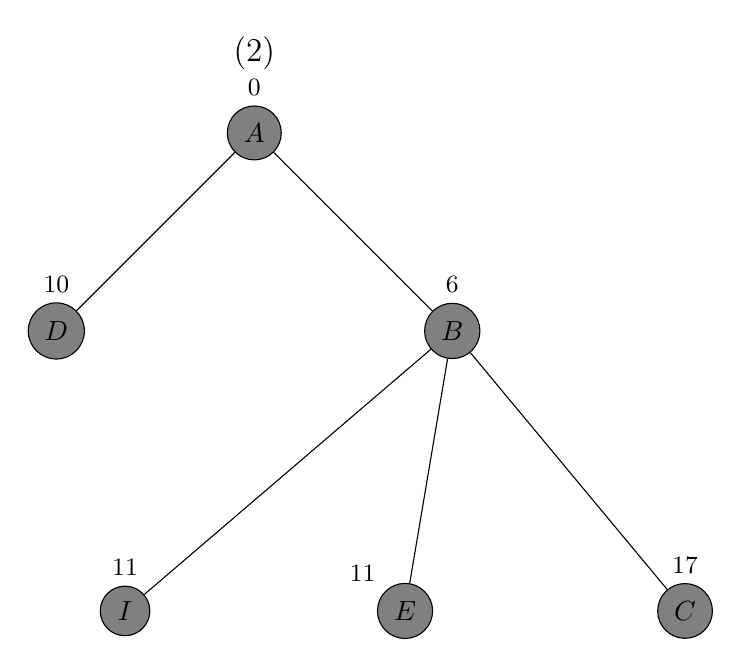
\begin{tikzpicture}
	\node[State, label={\small 0}] (A) {$A$};
	\node[State, below right of= A, label={\small 6}] (B) {$B$};
	\node[State, below left of= A, label={\small 10}] (D) {$D$};
	
	\node[State, below of= B, label={above left:\small 11}, xshift=-0.6cm] (E) {$E$};
	\node[State, right of= E, label={\small 17}] (C) {$C$};
	\node[State, left of= E, label={\small 11}] (I) {$I$};
	
	\draw[Edge] (A) -- (B);
	\draw[Edge] (A) -- (D);
	\draw[Edge] (B) -- (C);
	\draw[Edge] (B) -- (E);
	\draw[Edge] (B) -- (I);

	\node[label={[font=\large, align=center, name=aux1]above:{(2)}}, yshift=0.2cm] (text) at (A.north) {};
\end{tikzpicture}  & 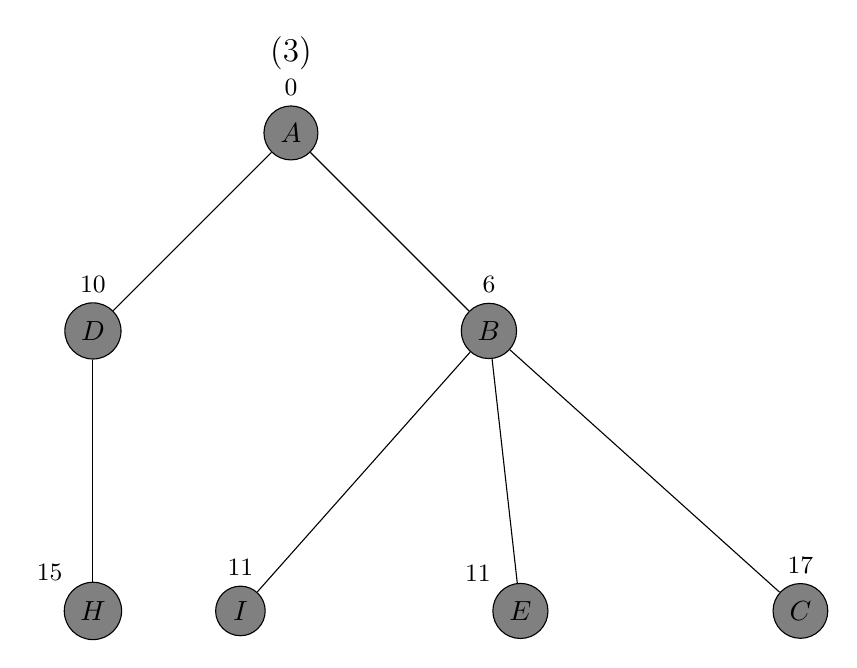
\begin{tikzpicture}
	\node[State, label={\small 0}] (A) {$A$};
	\node[State, below right of= A, label={\small 6}] (B) {$B$};
	\node[State, below left of= A, label={\small 10}] (D) {$D$};
	
	\node[State, below of= B, label={above left:\small 11}, xshift=0.4cm] (E) {$E$};
	\node[State, right of= E, label={\small 17}] (C) {$C$};
	\node[State, left of= E, label={\small 11}] (I) {$I$};

	\node[State, below of= D, label={above left:\small 15}] (H) {$H$};
	
	\draw[Edge] (A) -- (B);
	\draw[Edge] (A) -- (D);
	\draw[Edge] (B) -- (C);
	\draw[Edge] (B) -- (E);
	\draw[Edge] (B) -- (I);
	\draw[Edge] (D) -- (H);

	\node[label={[font=\large, align=center, name=aux1]above:{(3)}}, yshift=0.2cm] (text) at (A.north) {};
\end{tikzpicture}\\
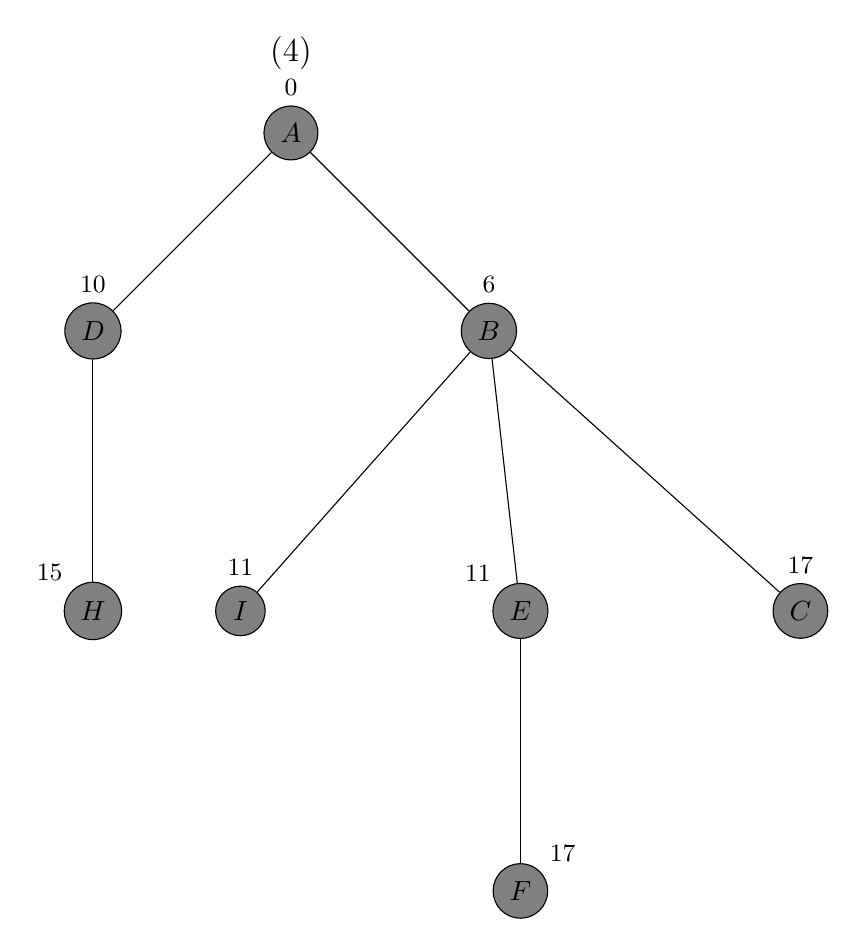
\begin{tikzpicture}
	\node[State, label={\small 0}] (A) {$A$};
	\node[State, below right of= A, label={\small 6}] (B) {$B$};
	\node[State, below left of= A, label={\small 10}] (D) {$D$};
	
	\node[State, below of= B, label={above left:\small 11}, xshift=0.4cm] (E) {$E$};
	\node[State, right of= E, label={\small 17}] (C) {$C$};
	\node[State, left of= E, label={\small 11}] (I) {$I$};

	\node[State, below of= D, label={above left:\small 15}] (H) {$H$};
	
	\node[State, below of= E, label={above right:\small 17}] (F) {$F$};
	\draw[Edge] (A) -- (B);
	\draw[Edge] (A) -- (D);
	\draw[Edge] (B) -- (C);
	\draw[Edge] (B) -- (E);
	\draw[Edge] (B) -- (I);
	\draw[Edge] (D) -- (H);
	\draw[Edge] (F) -- (E);

	\node[label={[font=\large, align=center, name=aux1]above:{(4)}}, yshift=0.2cm] (text) at (A.north) {};
\end{tikzpicture} & 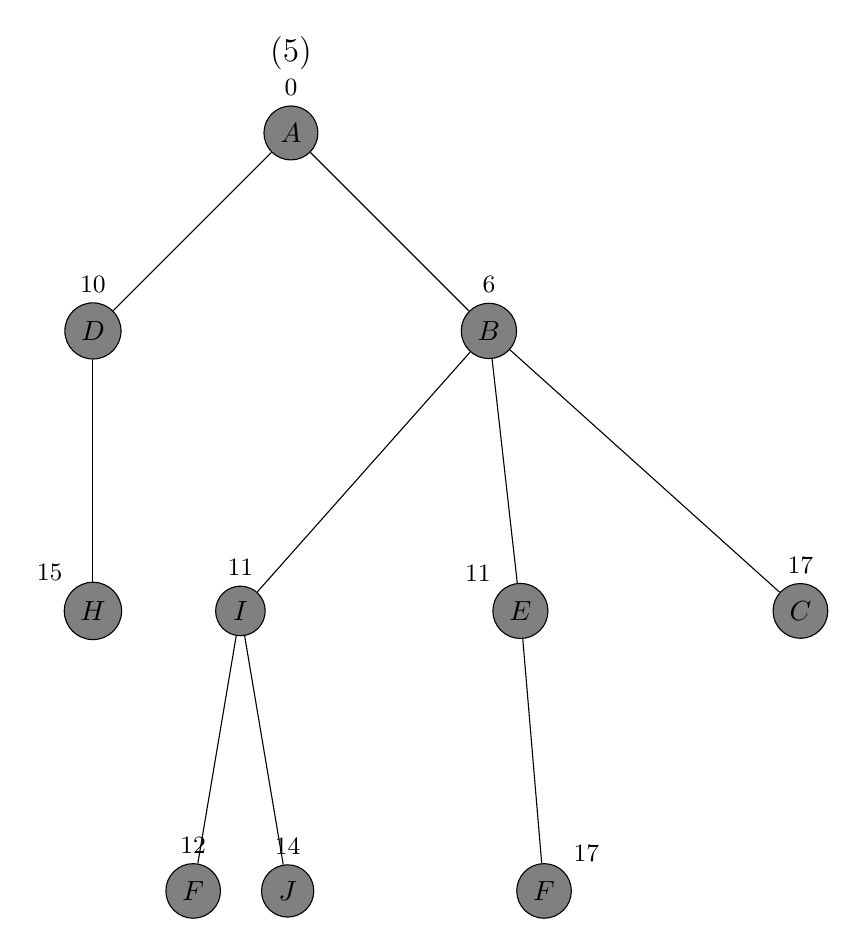
\begin{tikzpicture}
	\node[State, label={\small 0}] (A) {$A$};
	\node[State, below right of= A, label={\small 6}] (B) {$B$};
	\node[State, below left of= A, label={\small 10}] (D) {$D$};
	
	\node[State, below of= B, label={above left:\small 11}, xshift=0.4cm] (E) {$E$};
	\node[State, right of= E, label={\small 17}] (C) {$C$};
	\node[State, left of= E, label={\small 11}] (I) {$I$};

	\node[State, below of= D, label={above left:\small 15}] (H) {$H$};
	\node[State, below of= E, label={above right:\small 17}, xshift=0.3cm] (F) {$F$};
	\node[State, below of= I, label={\small 14}, xshift=0.6cm] (J) {$J$};
	\node[State, below of= I, label={\small 12}, xshift=-0.6cm] (F2) {$F$};
	\draw[Edge] (A) -- (B);
	\draw[Edge] (A) -- (D);
	\draw[Edge] (B) -- (C);
	\draw[Edge] (B) -- (E);
	\draw[Edge] (B) -- (I);
	\draw[Edge] (D) -- (H);
	\draw[Edge] (F) -- (E);
	\draw[Edge] (J) -- (I);
	\draw[Edge] (F2) -- (I);

	\node[label={[font=\large, align=center, name=aux1]above:{(5)}}, yshift=0.2cm] (text) at (A.north) {};
\end{tikzpicture} & 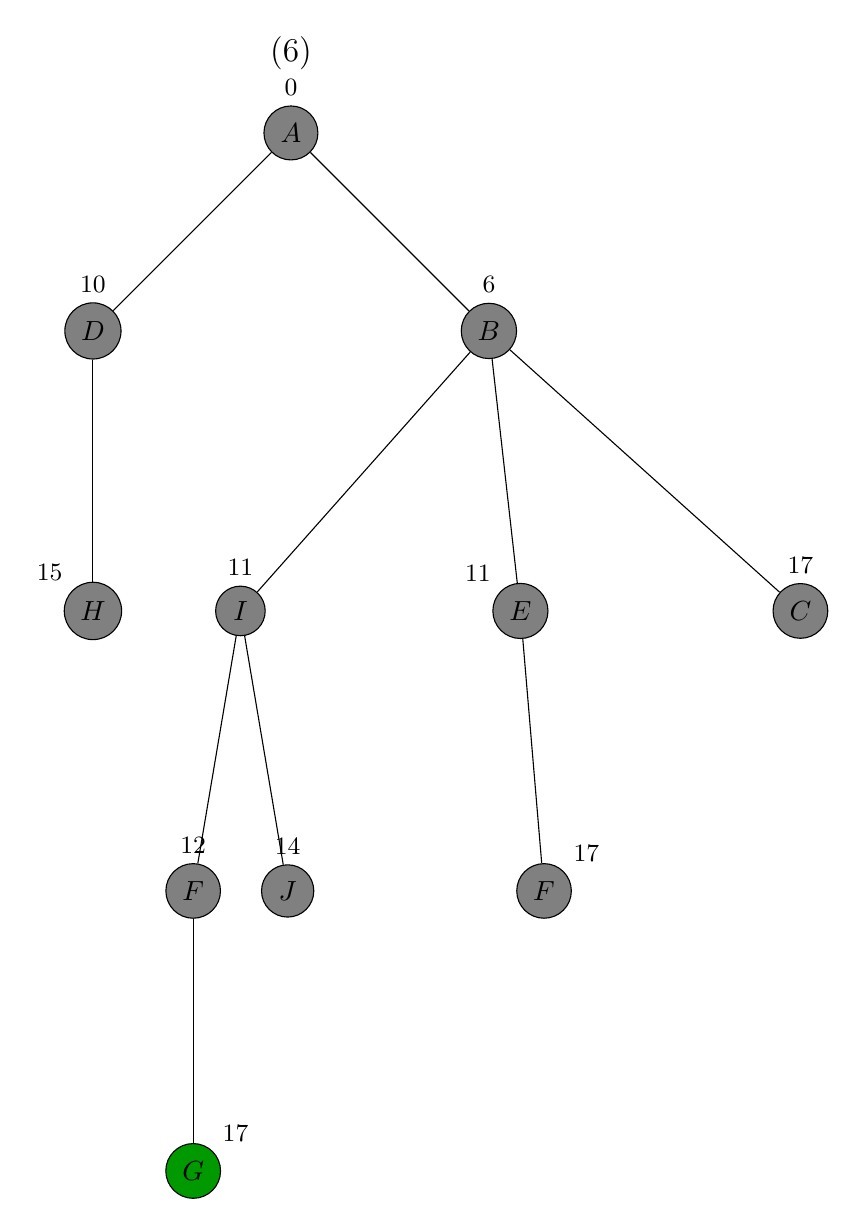
\begin{tikzpicture}
	\node[State, label={\small 0}] (A) {$A$};
	\node[State, below right of= A, label={\small 6}] (B) {$B$};
	\node[State, below left of= A, label={\small 10}] (D) {$D$};
	
	\node[State, below of= B, label={above left:\small 11}, xshift=0.4cm] (E) {$E$};
	\node[State, right of= E, label={\small 17}] (C) {$C$};
	\node[State, left of= E, label={\small 11}] (I) {$I$};

	\node[State, below of= D, label={above left:\small 15}] (H) {$H$};
	\node[State, below of= E, label={above right:\small 17}, xshift=0.3cm] (F) {$F$};
	\node[State, below of= I, label={\small 14}, xshift=0.6cm] (J) {$J$};
	\node[State, below of= I, label={\small 12}, xshift=-0.6cm] (F2) {$F$};
	\node[MarkedState, below of= F2, label={above right:\small 17}] (G) {$G$};

	\draw[Edge] (A) -- (B);
	\draw[Edge] (A) -- (D);
	\draw[Edge] (B) -- (C);
	\draw[Edge] (B) -- (E);
	\draw[Edge] (B) -- (I);
	\draw[Edge] (D) -- (H);
	\draw[Edge] (F) -- (E);
	\draw[Edge] (J) -- (I);
	\draw[Edge] (F2) -- (I);
	\draw[Edge] (F2) -- (G);

	\node[label={[font=\large, align=center, name=aux1]above:{(6)}}, yshift=0.2cm] (text) at (A.north) {};
\end{tikzpicture} \\
};
\end{tikzpicture}
\end{latin}

\end{document}